\section{Hybrid - Scalability}
\begin{frame}{Hybrid - Efficiency Results}
    \begin{table}[H]
        \centering
        \renewcommand{\arraystretch}{1.2}
        \setlength{\tabcolsep}{4pt}
        \footnotesize
        \begin{tabularx}{\textwidth}{c|*{7}{>{\centering\arraybackslash}X}}
            \hline
            \textbf{N\_Processes} & \textbf{0.033M} & \textbf{0.066M} & \textbf{0.131M} & \textbf{0.262M} & \textbf{0.524M} & \textbf{1.049M} & \textbf{2.097M} \\
            \hline
            1  & 1.000 & 1.000 & 1.000 & 1.000 & 1.000 & 1.000 & 1.000 \\
            2  & 1.040 & 0.975 & 0.984 & 0.985 & 0.968 & 1.029 & 0.840 \\
            4  & 1.075 & 1.057 & 0.970 & 1.068 & 0.955 & 1.052 & 0.929 \\
            8  & 1.055 & 0.981 & 0.978 & 1.000 & 0.996 & 1.038 & 0.907 \\
            16 & 1.003 & 0.929 & 0.880 & 0.893 & 0.915 & 0.923 & 0.860 \\
            32 & 0.974 & 0.872 & 0.828 & 0.970 & 0.888 & 0.903 & 0.822 \\
            64 & 0.925 & 0.862 & 0.854 & 0.922 & 0.912 & 0.897 & 0.868 \\
            \hline
        \end{tabularx}
        \caption{Efficiency for Hybrid approach for different dataset sizes and number of processes.}
    \label{tab:efficiency_hybrid}
    \end{table}
\end{frame}

% Graph showing efficiency results for Hybrid implementation
\begin{frame}{Hybrid - Efficiency Results}
    \begin{figure}[H]
        \centering
        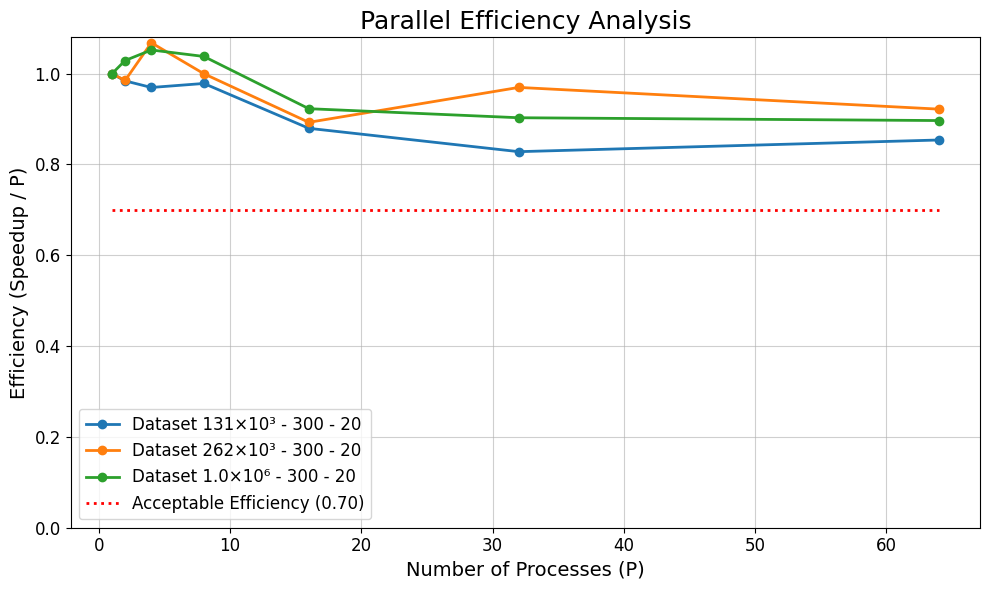
\includegraphics[width=0.8\textwidth]{../media/hybrid_efficiency.png}
        \caption{Hybrid Efficiency plot for different dataset sizes (small, medium, large). The dashed line indicates the target efficiency of 0.70.}
        \label{fig:hybrid_efficiency_plot}
    \end{figure}
\end{frame}

\begin{frame}{Hybrid - A more in depth look}
    \begin{minipage}{0.48\textwidth}
        \begin{figure}[H]
            \centering
            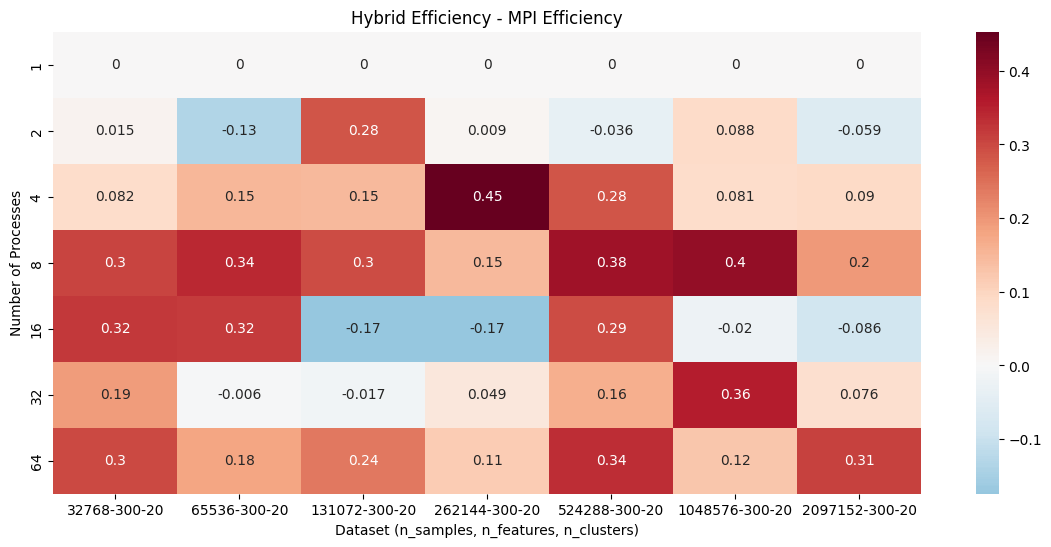
\includegraphics[width=1\textwidth]{../media/mstep_heatmap.png}
            \caption{M-Step Efficiency Heatmap for difference between Pure MPI and Hybrid approach. Red indicates higher efficiency in Hybrid, blue indicates higher efficiency in Pure MPI.}
            \label{fig:mstep_efficiency_heatmap}
        \end{figure}
    \end{minipage}
    \hfill
    \begin{minipage}{0.48\textwidth}
        \begin{figure}[H]
            \centering
            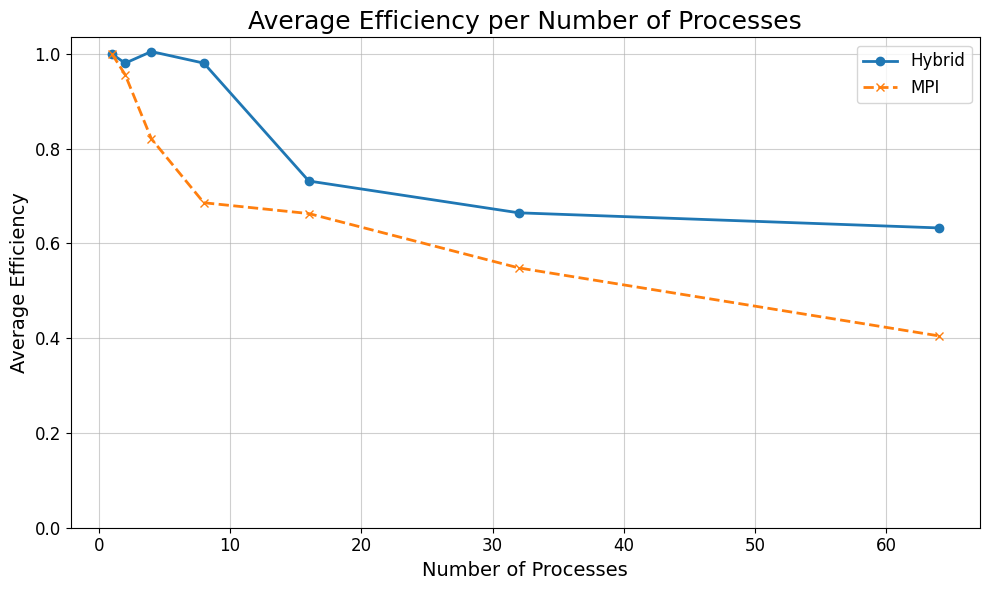
\includegraphics[width=1\textwidth]{../media/mstep_comparison.png}
            \caption{Average M-Step Efficiency Comparison between Pure MPI and Hybrid approach.}
            \label{fig:hybrid_speedup_plot}
        \end{figure}
    \end{minipage}
\end{frame}
